\section{Frameworks}
\textbf{Why Frameworks}
\begin{itemize}
    \item Avoid re-inventing the wheel
    \item It is easy but inefficient to program the same thing again and again
\end{itemize}
\vspace{10pt}
\textbf{What is a Framework}
\begin{itemize}
    \item \textcolor{blue}{Objekt-Orientierte Klassen die zusammenarbeiten} Viele Design Patterns sind Micro-Frameworks
    \item Framework bietet \textcolor{blue}{Hooks} für \textcolor{blue}{Extensions}
    \begin{itemize}
        \item Clients erweitern Framework Klassen oder Interfaces
        \item Semi-Komplette Lösung
    \end{itemize}
    \item Im Gegensatz zu einer Library, behaltet ein Framework den \textcolor{blue}{Kontrollfluss, nicht} die Extension-Komponente
    \begin{itemize}
        \item Inversion of Control via Callbacks: Dont call us, we call you!
        \item Kontrollfluss ist vom Framework zu den Applikations-Komponenten
    \end{itemize}
    \item Applikationen werden erstellt indem Framework-Komponenten erweitert werden
\end{itemize}
\vspace{10pt}
\textbf{Examples}

.NET Core, Entity Framework, React (lib), Vue

\subsubsection{Differences}
\textbf{Library}
\begin{itemize}
    \item Contain 3rd party Features which do not control the app flow (e.g. Math Library)
\end{itemize}
\vspace{10pt}
\textbf{Framework}
\begin{itemize}
    \item Provide Hooks / Extension points
    \item Strogly rely on Inversion of Control (IoC)
    \item Defines when hooks are called, thus controlls part of the app flow
\end{itemize}
\vspace{10pt}
\textbf{Application Framework}
\begin{itemize}
    \item Contains the \textit{main()} procedure
    \item Completely controls the app flow
\end{itemize}

\subsubsection{Consequences}

\textbf{Benefits}

\begin{itemize}
    \item Less code to write
    \item Reliable and robust code
    \item Consistent and modular code
    \item Reusability
    \item Maintenance
    \item More focus on areas of expertise, less focus on areas of system compatibility
    \item Generische Lösungen die andere wiederverwenden können
    \item \textcolor{blue}{Application Frameworks} bieten verbesserte Integration
\end{itemize}
\vspace{10pt}
\textbf{Liabilities}

\begin{itemize}
    \item \textcolor{blue}{Portability} Code ist stark gekoppelt zur überliegenden Framework
    \item \textcolor{blue}{Testability} Close coupling between framework parts
    \item \textcolor{blue}{Evolution} User's implementation may break due next
    Framework version
\end{itemize}


\subsection{Application Framework}
\begin{itemize}
    \item Objekt-Orientierte Klassen Library
    \item Main()-Methode lebt im \textcolor{blue}{Application Framework}
    \item Bietet \textcolor{blue}{Hooks} für die Erweiterung und \textcolor{blue}{Callbacks}
    \item Bietet ready-made Klassen für die Nutzung
    \item Erstellt eine Produktfamilie
    \item Wiederverwendung von Application Architekturen und Infrastrukturen
    \item Sehr hohe Qualitätsanforderungen an Application Frameworks
\end{itemize}
\vspace{10pt}
\textbf{Examples}

Spring, ASP.NET, Angular

\subsection{Micro Frameworks}

Hook Methods, Extension Point, Control Flow

\subsubsection{Solutions}

\textbf{Template Method}

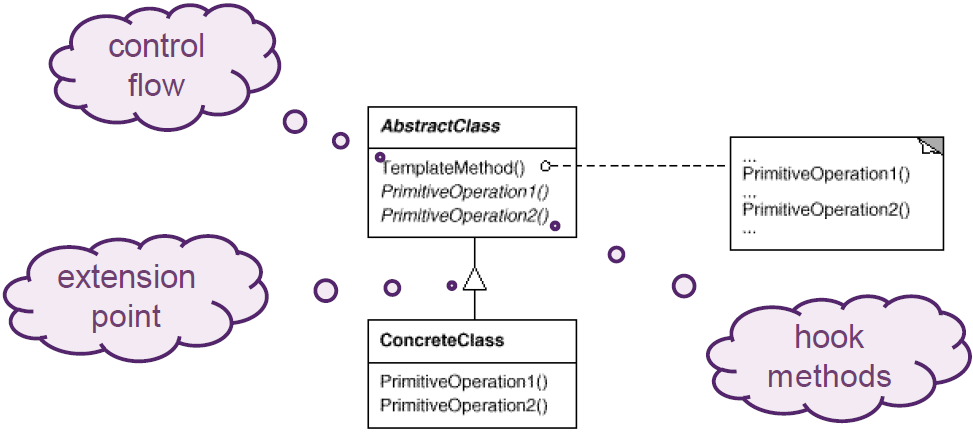
\includegraphics[width=\linewidth]{template_method_example.png} \\

\textbf{Strategy}

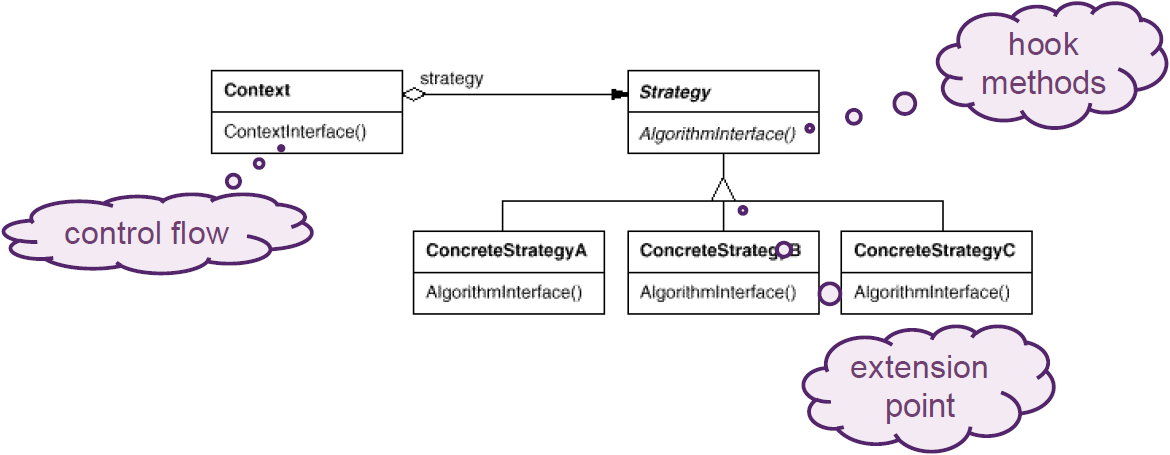
\includegraphics[width=\linewidth]{strategy_example.png} \\

\textbf{Command Processor}

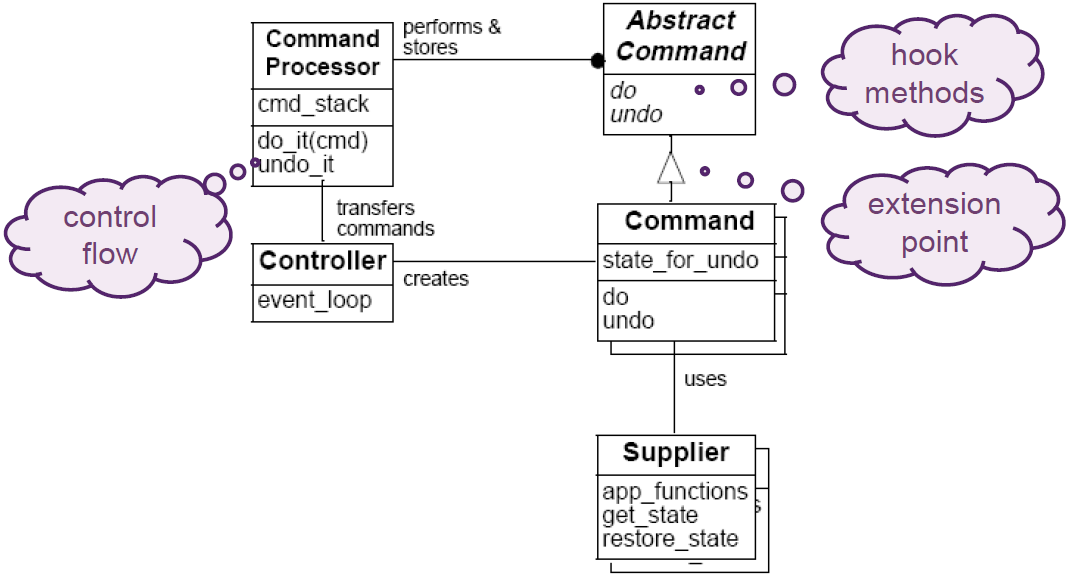
\includegraphics[width=\linewidth]{command_processor_example.png} \\

\vfill\null
\columnbreak

\textbf{Flyweight}

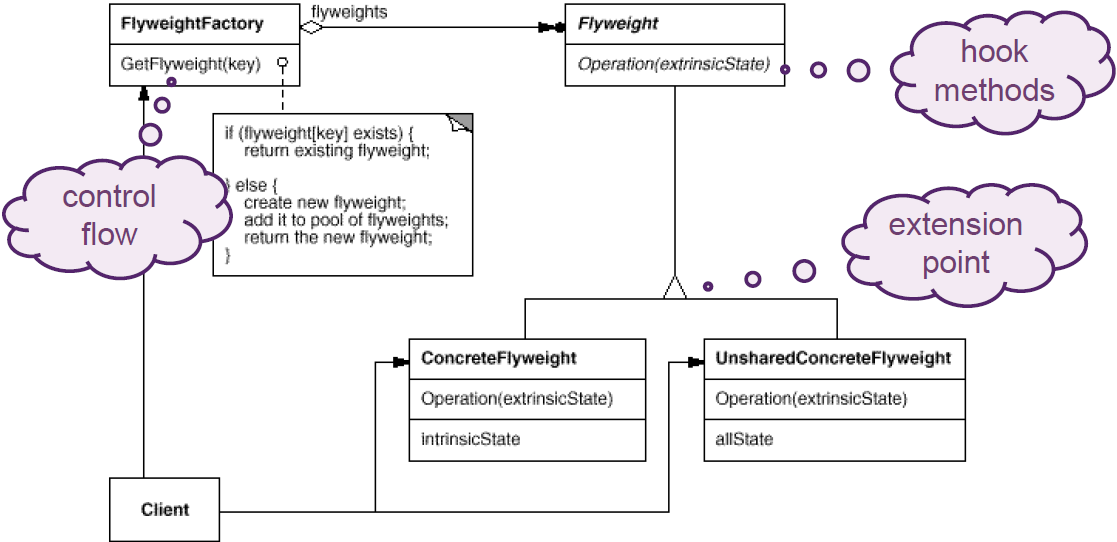
\includegraphics[width=\linewidth]{flyweight_hooks.png}

\subsection{Meta Frameworks}
A Framework for Evaluating Software Technology
\begin{itemize}
    \item Initial acquisition cost
    \item Long-term effect
    \item Training and support
    \item Future technoloy plans
    \item Response of direct competitor organizations
\end{itemize}
\vspace{10pt}
\textbf{Framework Evaluation Phases}

Keypoints

\begin{enumerate}
    \item understanding how the evaluated technology differs from other technologies; and
    \item understanding how these differences address the needs of specific usage contexts.
\end{enumerate}

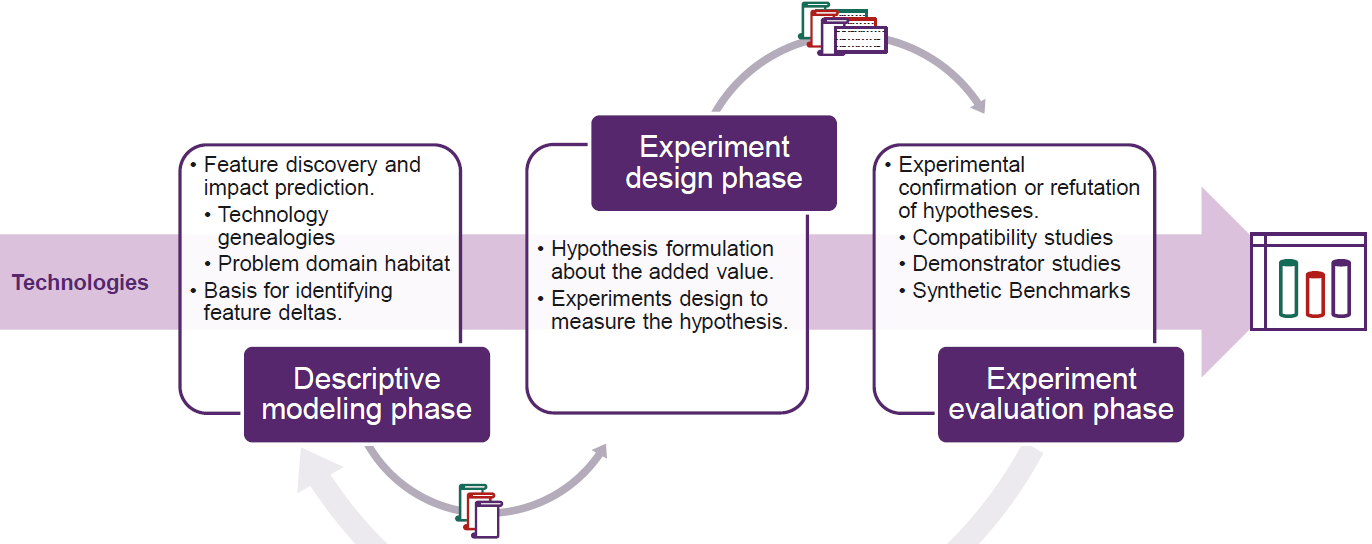
\includegraphics[width=\linewidth]{framework_eval.png}

\subsubsection{Frameworkers Dilemma}

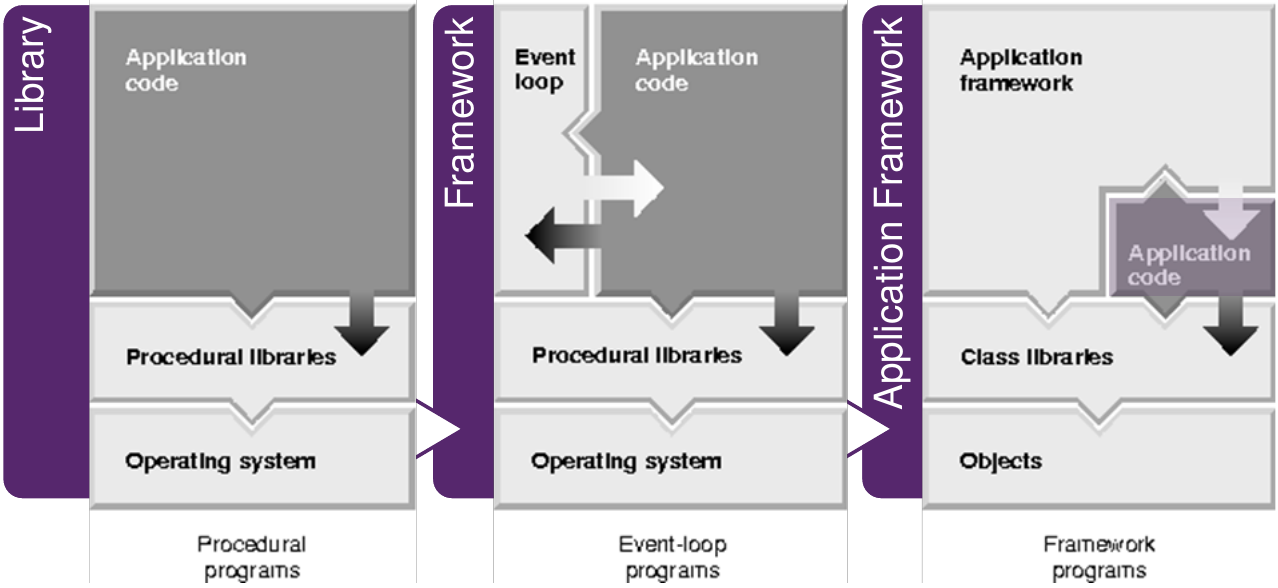
\includegraphics[width=\linewidth]{frameworkers-dilemma.png} \\

\textbf{Frameworkers Lock-In}

Beachte die funktionalen und nicht-funktionalen Anforderungen und evaluiere ein Framework mit Vorsicht, bevor \textit{locked-in}

\begin{itemize}
    \item Portability
    \item Testability
    \item Evolution
\end{itemize}
\vspace{10pt}

\vfill\null
\columnbreak

\textbf{Potential ways out of the dilemma}
\begin{enumerate}
    \item \textcolor{blue}{Denke vorab gut nach}
    \item \textcolor{blue}{Kümmere dich nicht zu sehr um die Benutzer des Frameworks} Stelle viele gute und nützliche neue Funktionen, die eine Portierung zu einem ''Muss'' machen, bereit
    \item \textcolor{blue}{Lass die Framework-Verwender mitmachen} Gebe Benutzer Zeit zum migrieren (deprecated interfaces), backward compatibility, simple and flexible interfaces (Bsp. Convention over Configuration), configurability (reduziere Code-Abhängigkeiten)
    \item \textcolor{blue}{Verwende unterstützende Technologien}
\end{enumerate}

\subsection{Discussion}

\textbf{Why is evolution of frameworks so challenging?}

There are two reasons for lack of framework evolution and improvement
\begin{enumerate}
    \item no application uses the framework
    \begin{itemize}
        \item no users, no need to improve or evolve
        \item no experience on what to improve
    \end{itemize}
    \item one or more applications use the framework
    \begin{itemize}
        \item changing the framework risks breaking applications
        \item applications produce work-arounds to framework deficiencies (Mängel)
    \end{itemize}
\end{enumerate}
